% $Id: template.tex 11 2007-04-03 22:25:53Z jpeltier $

\documentclass{vgtc}                          % final (conference style)
%\documentclass[review]{vgtc}                 % review
%\documentclass[widereview]{vgtc}             % wide-spaced review
%\documentclass[preprint]{vgtc}               % preprint
%\documentclass[electronic]{vgtc}             % electronic version

%% Uncomment one of the lines above depending on where your paper is
%% in the conference process. ``review'' and ``widereview'' are for review
%% submission, ``preprint'' is for pre-publication, and the final version
%% doesn't use a specific qualifier. Further, ``electronic'' includes
%% hyperreferences for more convenient online viewing.

%% Please use one of the ``review'' options in combination with the
%% assigned online id (see below) ONLY if your paper uses a double blind
%% review process. Some conferences, like IEEE Vis and InfoVis, have NOT
%% in the past.

%% Figures should be in CMYK or Grey scale format, otherwise, colour 
%% shifting may occur during the printing process.

%% These few lines make a distinction between latex and pdflatex calls and they
%% bring in essential packages for graphics and font handling.
%% Note that due to the \DeclareGraphicsExtensions{} call it is no longer necessary
%% to provide the the path and extension of a graphics file:
%% \includegraphics{diamondrule} is completely sufficient.
%%
\ifpdf%                                % if we use pdflatex
  \pdfoutput=1\relax                   % create PDFs from pdfLaTeX
  \pdfcompresslevel=9                  % PDF Compression
  \pdfoptionpdfminorversion=7          % create PDF 1.7
  \ExecuteOptions{pdftex}
  \usepackage{graphicx}                % allow us to embed graphics files
  \DeclareGraphicsExtensions{.pdf,.png,.jpg,.jpeg} % for pdflatex we expect .pdf, .png, or .jpg files
\else%                                 % else we use pure latex
  \ExecuteOptions{dvips}
  \usepackage{graphicx}                % allow us to embed graphics files
  \DeclareGraphicsExtensions{.eps}     % for pure latex we expect eps files
\fi%

%% it is recomended to use ``\autoref{sec:bla}'' instead of ``Fig.~\ref{sec:bla}''
\graphicspath{{figures/}{pictures/}{images/}{./}} % where to search for the images

\usepackage{microtype}                 % use micro-typography (slightly more compact, better to read)
\PassOptionsToPackage{warn}{textcomp}  % to address font issues with \textrightarrow
\usepackage{textcomp}                  % use better special symbols
\usepackage{mathptmx}                  % use matching math font
\usepackage{times}                     % we use Times as the main font
\renewcommand*\ttdefault{txtt}         % a nicer typewriter font
\usepackage{cite}                      % needed to automatically sort the references
\usepackage{tabu}                      % only used for the table example
\usepackage{booktabs}                  % only used for the table example
%% We encourage the use of mathptmx for consistent usage of times font
%% throughout the proceedings. However, if you encounter conflicts
%% with other math-related packages, you may want to disable it.


%% If you are submitting a paper to a conference for review with a double
%% blind reviewing process, please replace the value ``0'' below with your
%% OnlineID. Otherwise, you may safely leave it at ``0''.
\onlineid{0}

%% declare the category of your paper, only shown in review mode
\vgtccategory{Research}

%% allow for this line if you want the electronic option to work properly
\vgtcinsertpkg

%% In preprint mode you may define your own headline. If not, the default IEEE copyright message will appear in preprint mode.
%\preprinttext{To appear in an IEEE VGTC sponsored conference.}

%% This adds a link to the version of the paper on IEEEXplore
%% Uncomment this line when you produce a preprint version of the article 
%% after the article receives a DOI for the paper from IEEE
%\ieeedoi{xx.xxxx/TVCG.201x.xxxxxxx}


%% Paper title.

\title{Interactive Visualization of Multivariate Clinical Data in Force Graph}

%% This is how authors are specified in the conference style

%% Author and Affiliation (single author).
%%\author{Roy G. Biv\thanks{e-mail: roy.g.biv@aol.com}}
%%\affiliation{\scriptsize Allied Widgets Research}

%% Author and Affiliation (multiple authors with single affiliations).
%%\author{Roy G. Biv\thanks{e-mail: roy.g.biv@aol.com} %
%%\and Ed Grimley\thanks{e-mail:ed.grimley@aol.com} %
%%\and Martha Stewart\thanks{e-mail:martha.stewart@marthastewart.com}}
%%\affiliation{\scriptsize Martha Stewart Enterprises \\ Microsoft Research}

%% Author and Affiliation (multiple authors with multiple affiliations)
\author{Mingi Ryu\thanks{e-mail: mingir2@illinois.edu}\\ %
        \scriptsize University of Illinois at Urbana-Champaign %
     \parbox{1.4in}{\scriptsize \centering}}

%% A teaser figure can be included as follows, but is not recommended since
%% the space is now taken up by a full width abstract.
%\teaser{
%  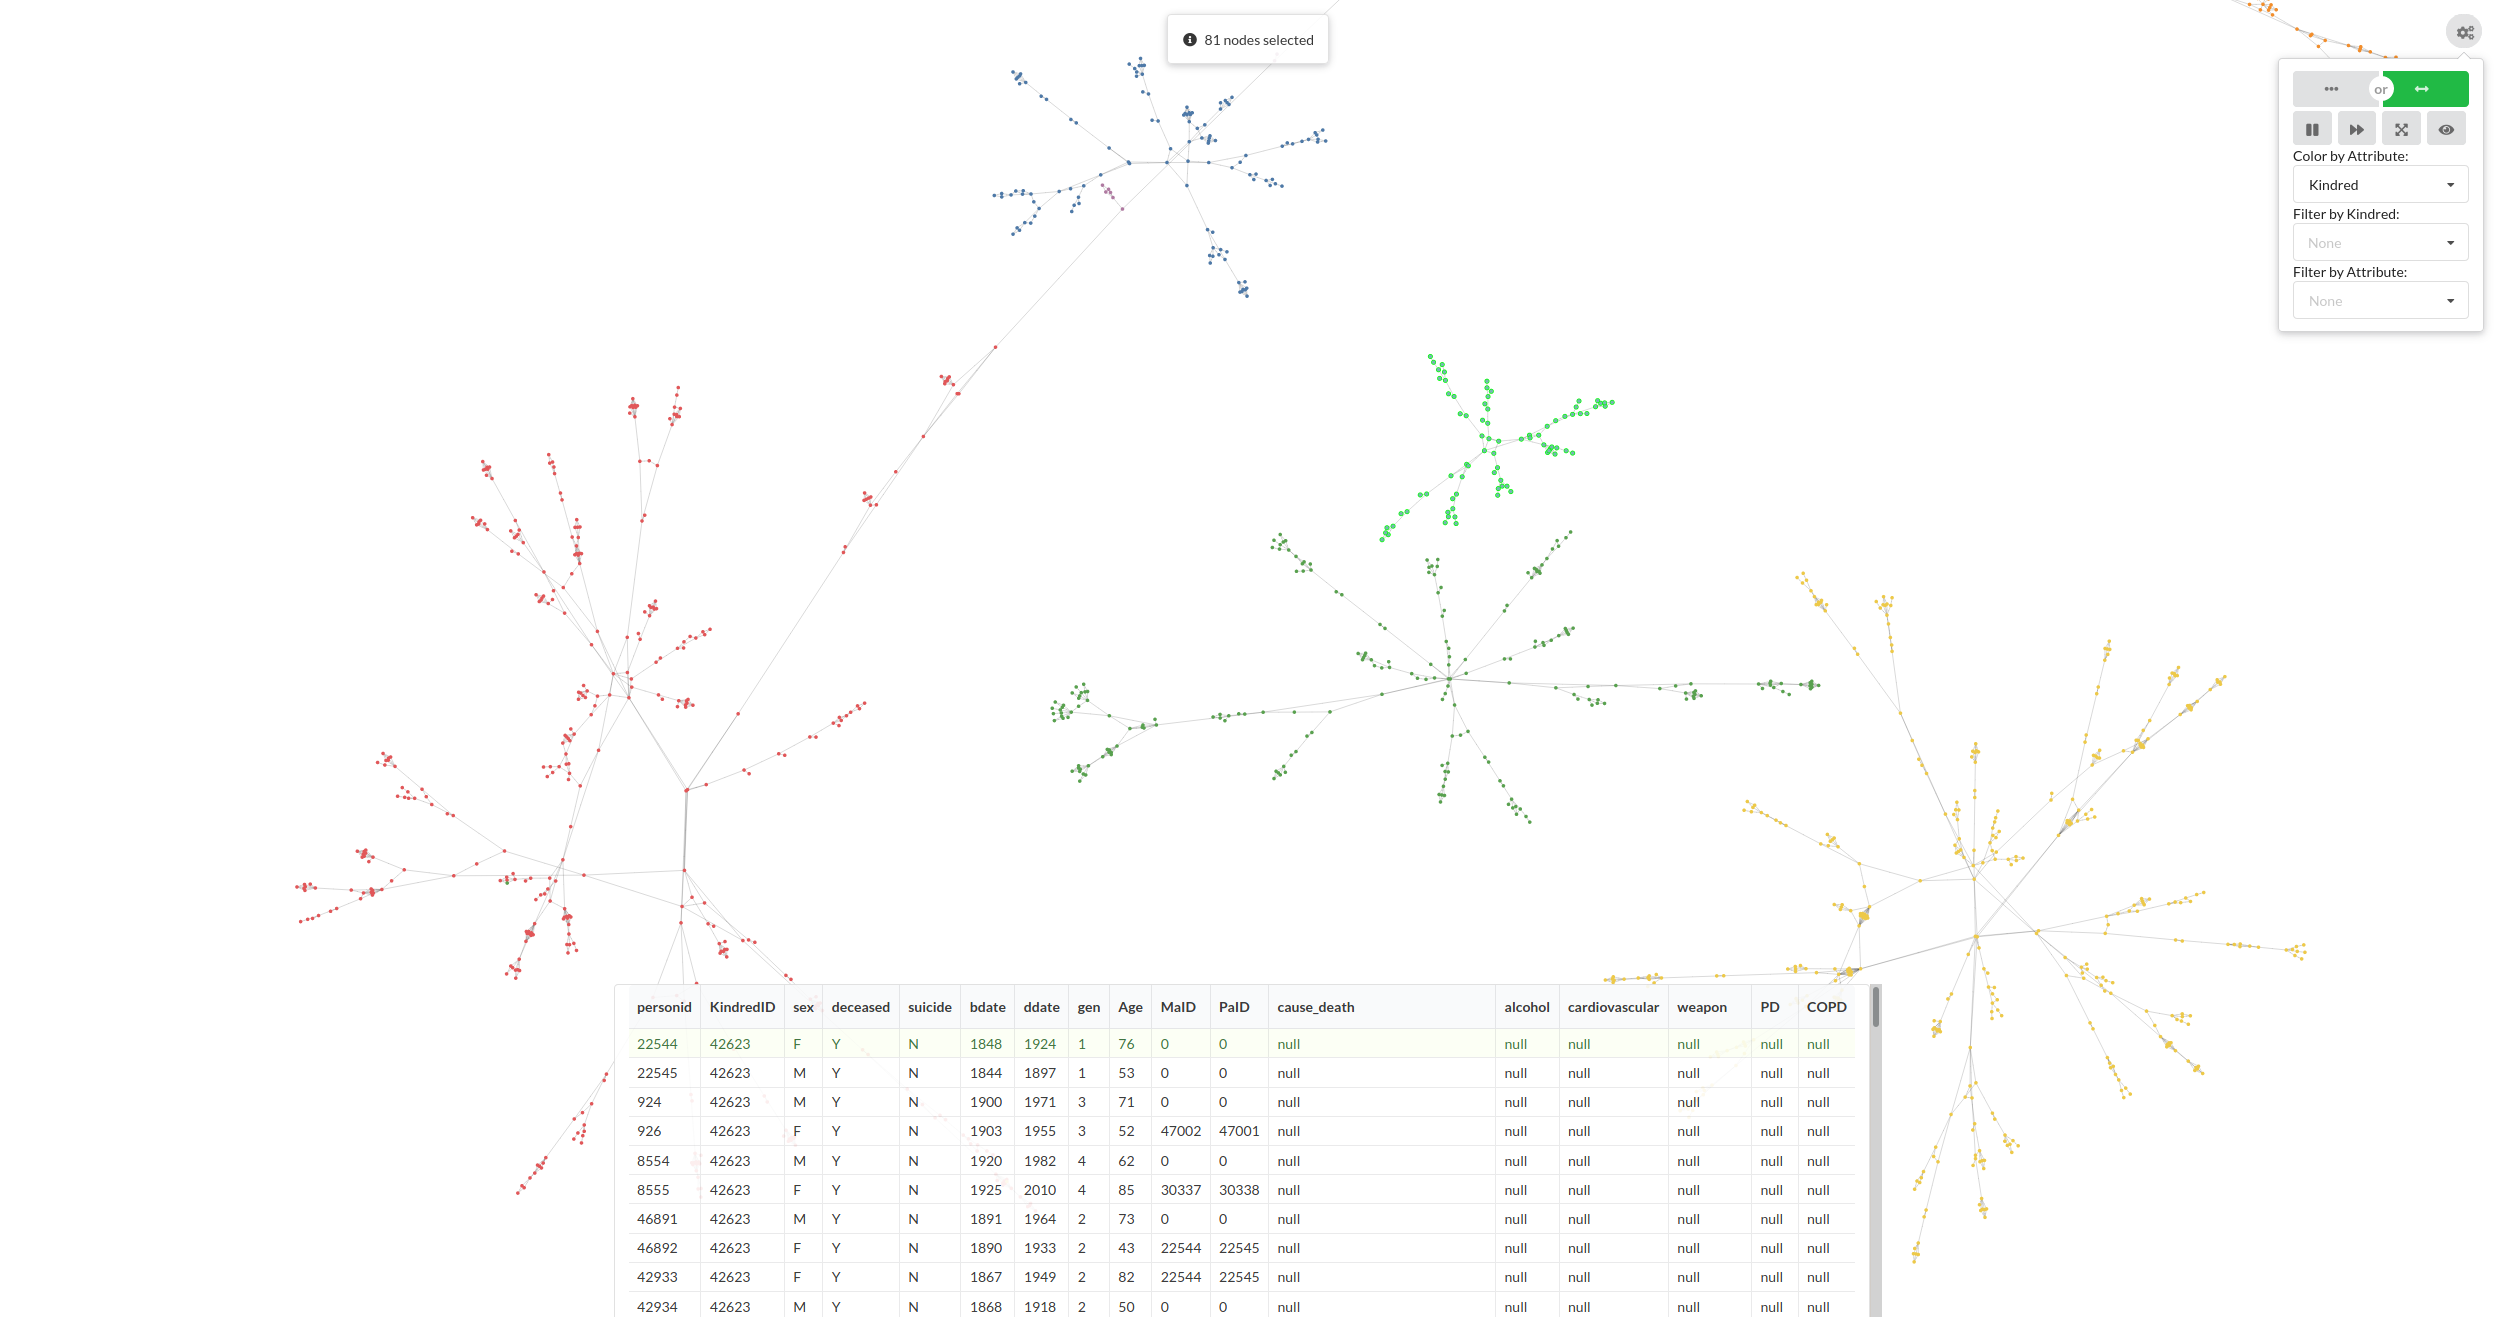
\includegraphics[width=\textwidth]{pictures/splash.png}
%  \caption{Lookit! Lookit!}
%}

%% Abstract section.
\abstract{Visualization of structure and multivariate data are often correlated, yet remains a major challenge. Recent advances in graph visualization have introduced domain-specific visualizations that are mostly tailored for domain experts. This paper introduces a web-based application where a basic set of interaction and visualization techniques is used to perform visualization tasks.  %
} % end of abstract

%% ACM Computing Classification System (CCS). 
%% See <http://www.acm.org/about/class> for details.
%% We recommend the 2012 system <http://www.acm.org/about/class/class/2012>
%% For the 2012 system use the ``\CCScatTwelve'' which command takes four arguments.
%% The 1998 system <http://www.acm.org/about/class/class/2012> is still possible
%% For the 1998 system use the ``\CCScat'' which command takes four arguments.
%% In both cases the last two arguments (1998) or last three (2012) can be empty.

\CCScatlist{
  \CCScatTwelve{Human-centered Computing}{Visualization}{}{},
  \CCScatTwelve{Force-directed Graph}{}{}{},
  \CCScatTwelve{Multivariate networks}{}{}{}
}

%\CCScatlist{
  %\CCScat{H.5.2}{User Interfaces}{User Interfaces}{Graphical user interfaces (GUI)}{};
  %\CCScat{H.5.m}{Information Interfaces and Presentation}{Miscellaneous}{}{}
%}

%% Copyright space is enabled by default as required by guidelines.
%% It is disabled by the 'review' option or via the following command:
% \nocopyrightspace

%%%%%%%%%%%%%%%%%%%%%%%%%%%%%%%%%%%%%%%%%%%%%%%%%%%%%%%%%%%%%%%%
%%%%%%%%%%%%%%%%%%%%%% START OF THE PAPER %%%%%%%%%%%%%%%%%%%%%%
%%%%%%%%%%%%%%%%%%%%%%%%%%%%%%%%%%%%%%%%%%%%%%%%%%%%%%%%%%%%%%%%%

\begin{document}

%% The ``\maketitle'' command must be the first command after the
%% ``\begin{document}'' command. It prepares and prints the title block.

%% the only exception to this rule is the \firstsection command
\firstsection{Introduction}

\maketitle

%% \section{Introduction} %for journal use above \firstsection{..} instead

As an alternative to the hierarchical graph used by Lineage~\cite{Nobre:2018:VMC}, force graph is used to visualize the dataset without additional abstractions. Nevertheless, force-directed graph runs the risk of "hairball-like" visualization due to overdraw and clutter~\cite{Elzen:2014:DOSA}, while the hierarchical graph retains a consistent layout and most of the topology via decycling and linearization~\cite{Nobre:2018:VMC}.

To address the possible overdraw and clutter, the application uses an interactive force graph framework created by Vasco Asturiano. force-graph is a web component to represent a graph data structure in a 2-dimensional canvas using HTML5 canvas for rendering and d3-force  for the underlying physics engine~\cite{Asturiano:2018:FG}. It supports a core set of features such as node-link selections, colored nodes, directional links, view manipulation, and more as an interactive framework.  

%The four tasks outlined in the BioVis@IEEE Challenges Workshop are carried out and described using the Graph Task Taxonomy~\cite{Lee:2006:TTGV}. 

\section{Dataset and Implementation}

The dataset provide a sample of 10 families in the Utah Population Database that have a high incidence of suicide, as defined by their FSIR (Family Suicide Incidence Ratio)~\cite{BioVis:2020:WS}. It provides information on the topology of the families, and each data point has a list of approximately 30 demographic and clinical attributes.

To make full use of the dataset, attributes and structure datasets were combined into a single dataset by joining on the "personid" field. Because the "personid" field contained duplicates with different attribute values, only the first instance of the duplicate was stored in the final dataset and no form of aggregation was made to merge the duplicates.

Since the force-graph framework utilizes d3-force library to visualize the graph data, the dataset was converted from rows and columns to nodes and links format. For this particular dataset, a single row corresponds to a single node and a single directed link represents the relationship between a parent and a child. In addition, not all 30 attributes were included since certain attributes did not provide useful information (race and location) or were essentially redundant (AgeID- and Nr.Diag-).

While the key component of the application is the force-graph, a significant amount of JavaScript, HTML, and CSS was written for the implementation of interactive components. In addition, the Semantic UI framework was used for the modern look and responsive design. For more details, the code can be found on GitHub. https:/github.com/mingir2/ten-families-graph/ 

\section{Tasks and Results}

To better understand the outlined tasks~\cite{BioVis:2020:WS}, the Graph Task Taxonomy was used to dissect the four high-level task into a set of broader low-level tasks~\cite{Lee:2006:TTGV}. Within each paragraph, each high-level task is broken down into a set of tasks, followed by an example figure for further clarification.

\subsection{Co-occurrence}

\begin{itemize}
\item{For a given target individual, identify similar cases, including
how they are related amongst themselves (such as whether they co-occur
in a given family.}
\end{itemize}

Given that the individual has an attribute of interest, a topology-based task may be used to identify similar cases and co-occurrence in a family. As such, the task is broken down into the following set of tasks: [Find on Nodes + Filter on Nodes + Retrieve Value on Nodes + Scan on Nodes + Find Adjacent Nodes on Nodes].

In \autoref{fig:occurrence}, an individual is chosen based on suicide cases with female attribute. In order to identify similar cases, the graph filtered by female attribute and colored by suicide cases. Then, the graph is scanned to locate any sub-graphs with co-occurrence.

\begin{figure}[tb]
 \centering % avoid the use of \begin{center}...\end{center} and use \centering instead (more compact)
 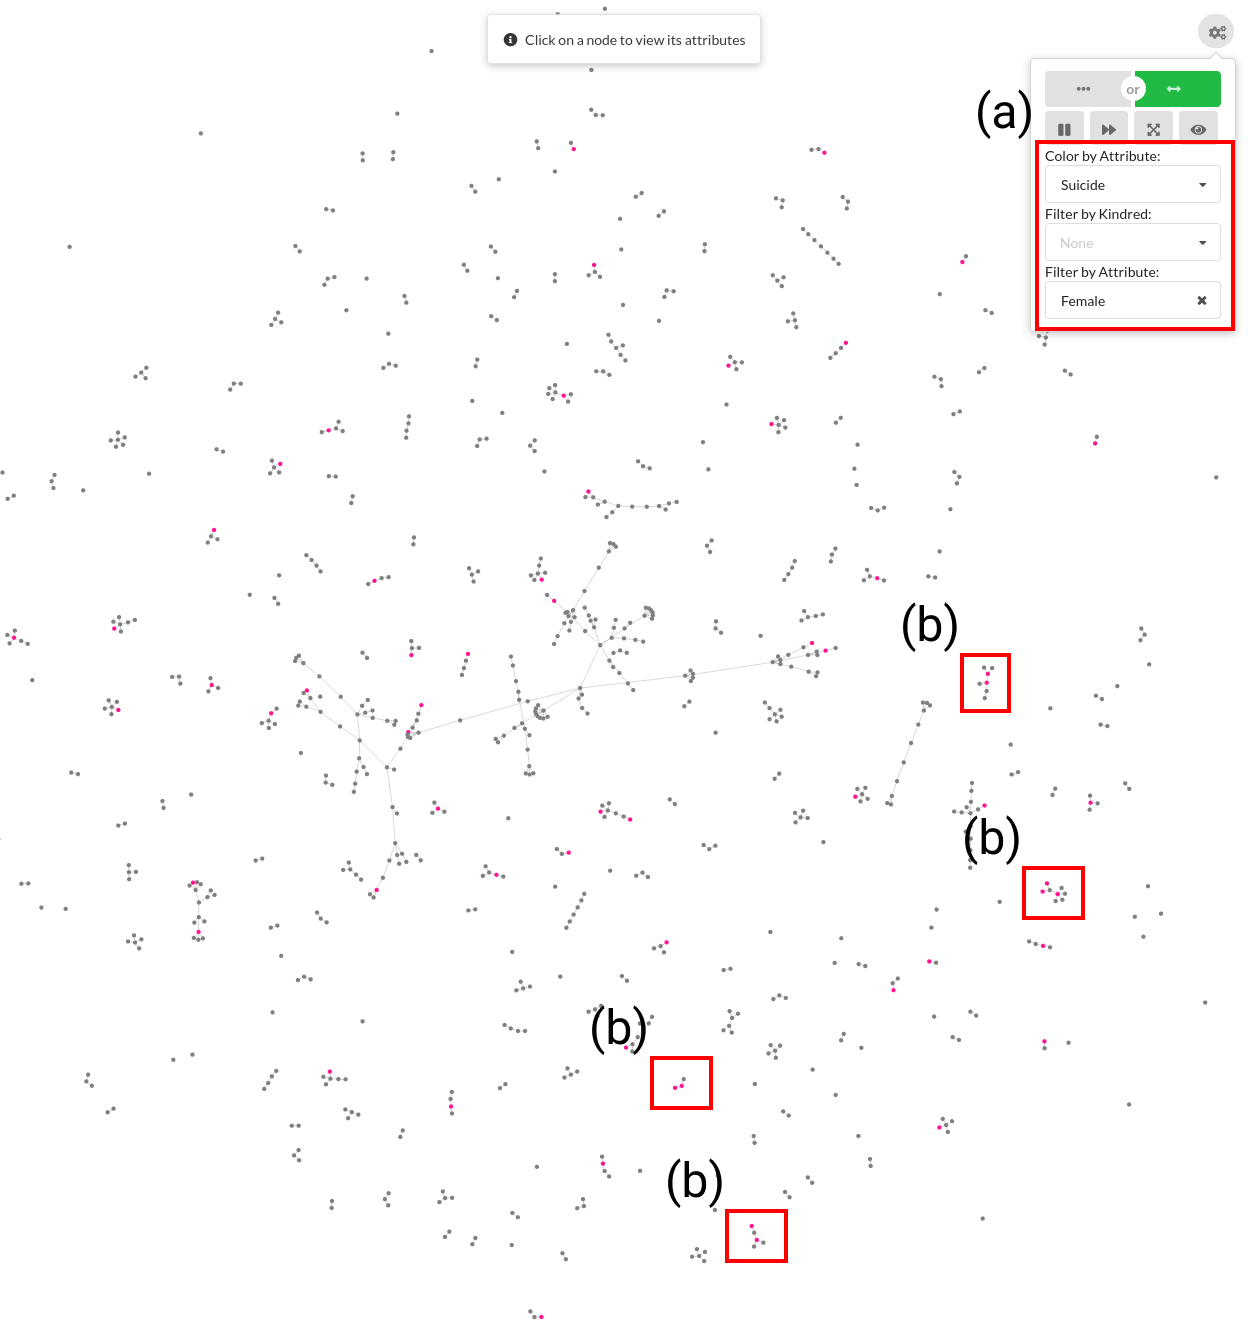
\includegraphics[width=\columnwidth]{pictures/occurrence.png}
 \caption{A graph of suicide cases with female attribute. (a) Colored by suicide cases and filtered by female attribute. (b) Sub-graphs with co-occurrence of suicide cases with female attribute.}
 \label{fig:occurrence}
\end{figure}

\subsection{Distribution}

\begin{itemize}
\item{Characterize the distribution of clinical attributes for suicide cases in families with high incidence ratios (high relative number of cases).}
\end{itemize}

When characterizing a distribution, a much broader range of low-level tasks may be used to represent both the topology and the attributes. Because the graph needs to be filtered based on multiple attributes, the following set of tasks are used: [Find on Nodes + Filter on Nodes + Retrieve Value on Nodes + Count on Nodes + Filter on Nodes + Retrieve Value on Nodes + Scan on Nodes].

In \autoref{fig:distribution}, the number of suicide cases are counted by filtering suicide cases and selecting all the nodes within the graph. Then, the graph is filtered by family group where the nodes are colored by cardiovascular attribute.

\begin{figure}[tb]
 \centering % avoid the use of \begin{center}...\end{center} and use \centering instead (more compact)
 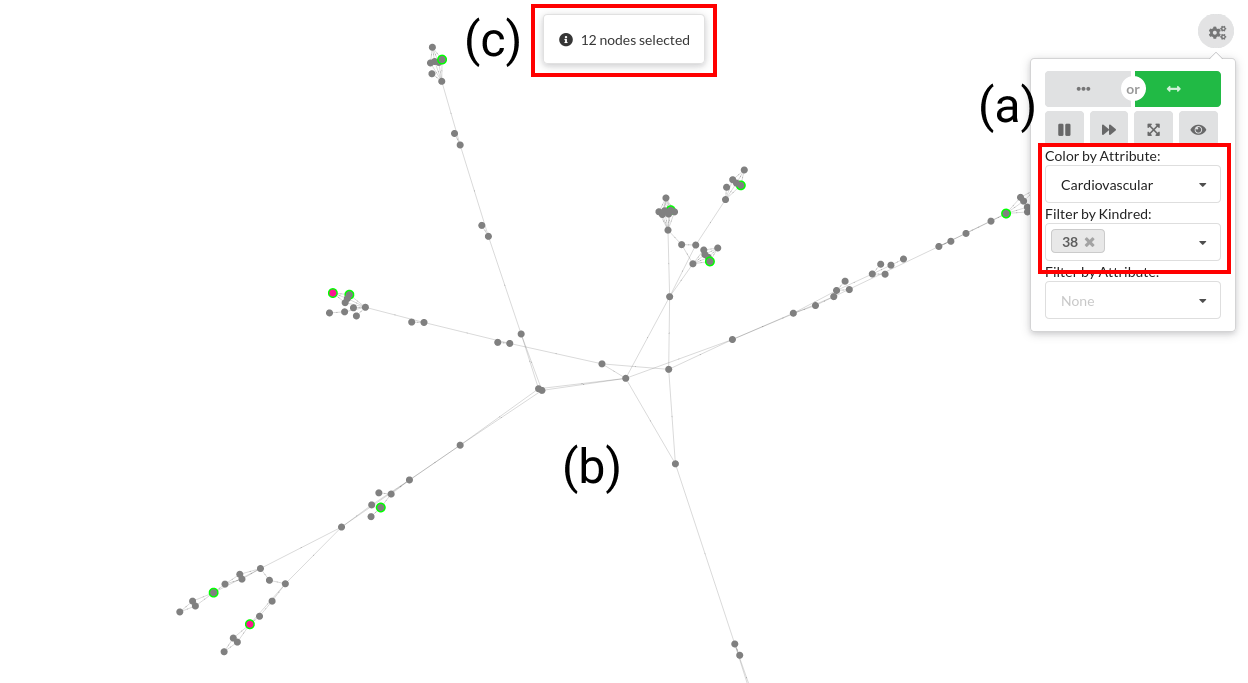
\includegraphics[width=\columnwidth]{pictures/distribution.png}
 \caption{A graph of family 38 with 12 suicide cases selected. (a) Colored by cardiovascular attribute and filtered by family 38. (b) Selected nodes are highlighted in green. (c) Number of nodes selected, which corresponds to the number of suicide cases in family 38.}
 \label{fig:distribution}
\end{figure}

\subsection{Relationship}

\begin{itemize}
\item{Characterize (i.e, the relationship between cases and their attributes) suicide cases in families with high incidences of a given clinical attribute (such as depression).}
\end{itemize}

This task is relatively trivial and may be broken down into the following set of tasks: [Find on Nodes + Filter on Nodes + Retrieve Value on Nodes + Scan on Nodes].

In \autoref{fig:relationship}, the graph is filtered based on depression attribute and colored by suicide cases to illustrate the relationship between the attribute and the cases.

\begin{figure}[tb]
 \centering % avoid the use of \begin{center}...\end{center} and use \centering instead (more compact)
 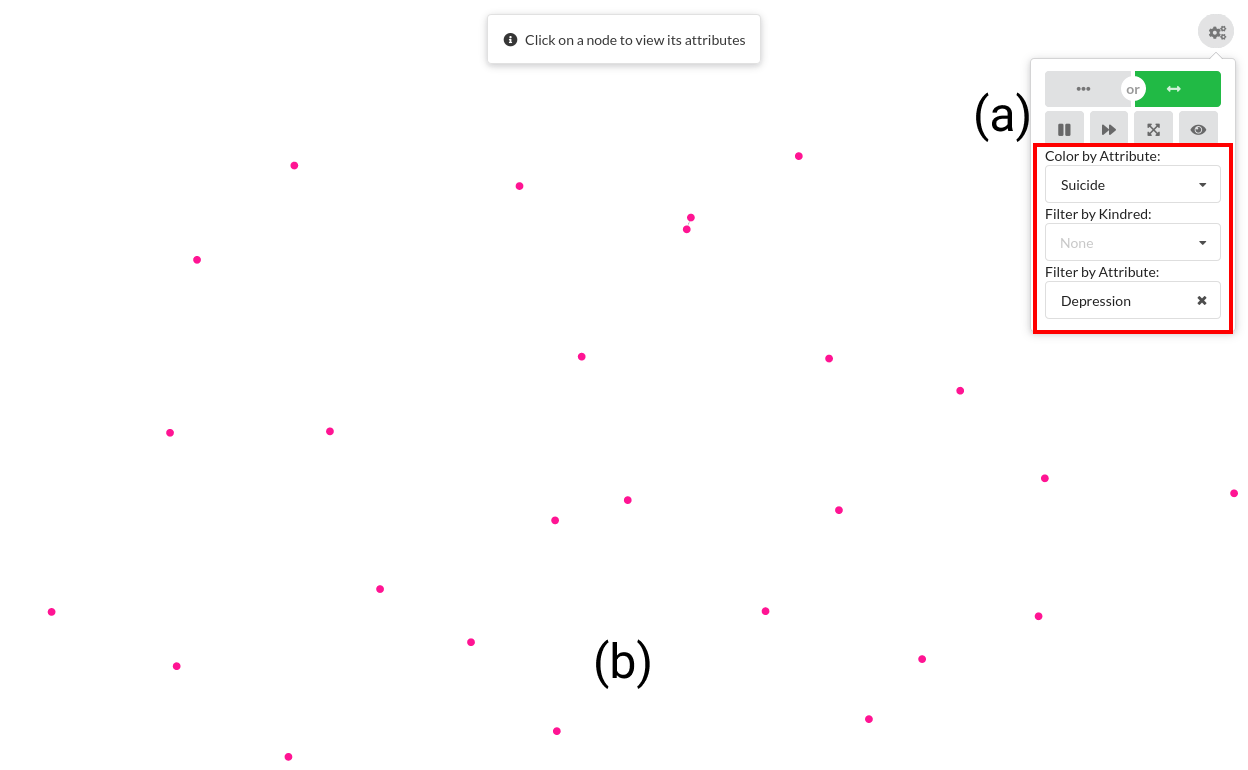
\includegraphics[width=\columnwidth]{pictures/relationship.png}
 \caption{A graph of relationship between depression and suicide. (a) Colored by suicide cases and filtered by depression attribute. (b) While this figure shows that each person with depression has committed suicide, the contrary is not necessarily true. Not every person who has committed suicide was also in depression.}
 \label{fig:relationship}
\end{figure}

\subsection{Comparison}

\begin{itemize}
\item{Compare clinical information for suicide cases with their immediate relatives (siblings, parents, and children). }
\end{itemize}

In order to compare clinical information of immediate relatives, a person of interest must first be identified and the relevant cases may then be selected for a detailed comparison. The task may be defined as follows: [Find on Nodes + Find Adjacent Nodes on Nodes + Retrieve Value on Nodes].

In \autoref{fig:comparison}, the siblings (adjacent nodes) are selected to compare clinical attributes. In this case, there are 2 suicide cases of similar age, but of different genders.

\begin{figure}[tb]
 \centering % avoid the use of \begin{center}...\end{center} and use \centering instead (more compact)
 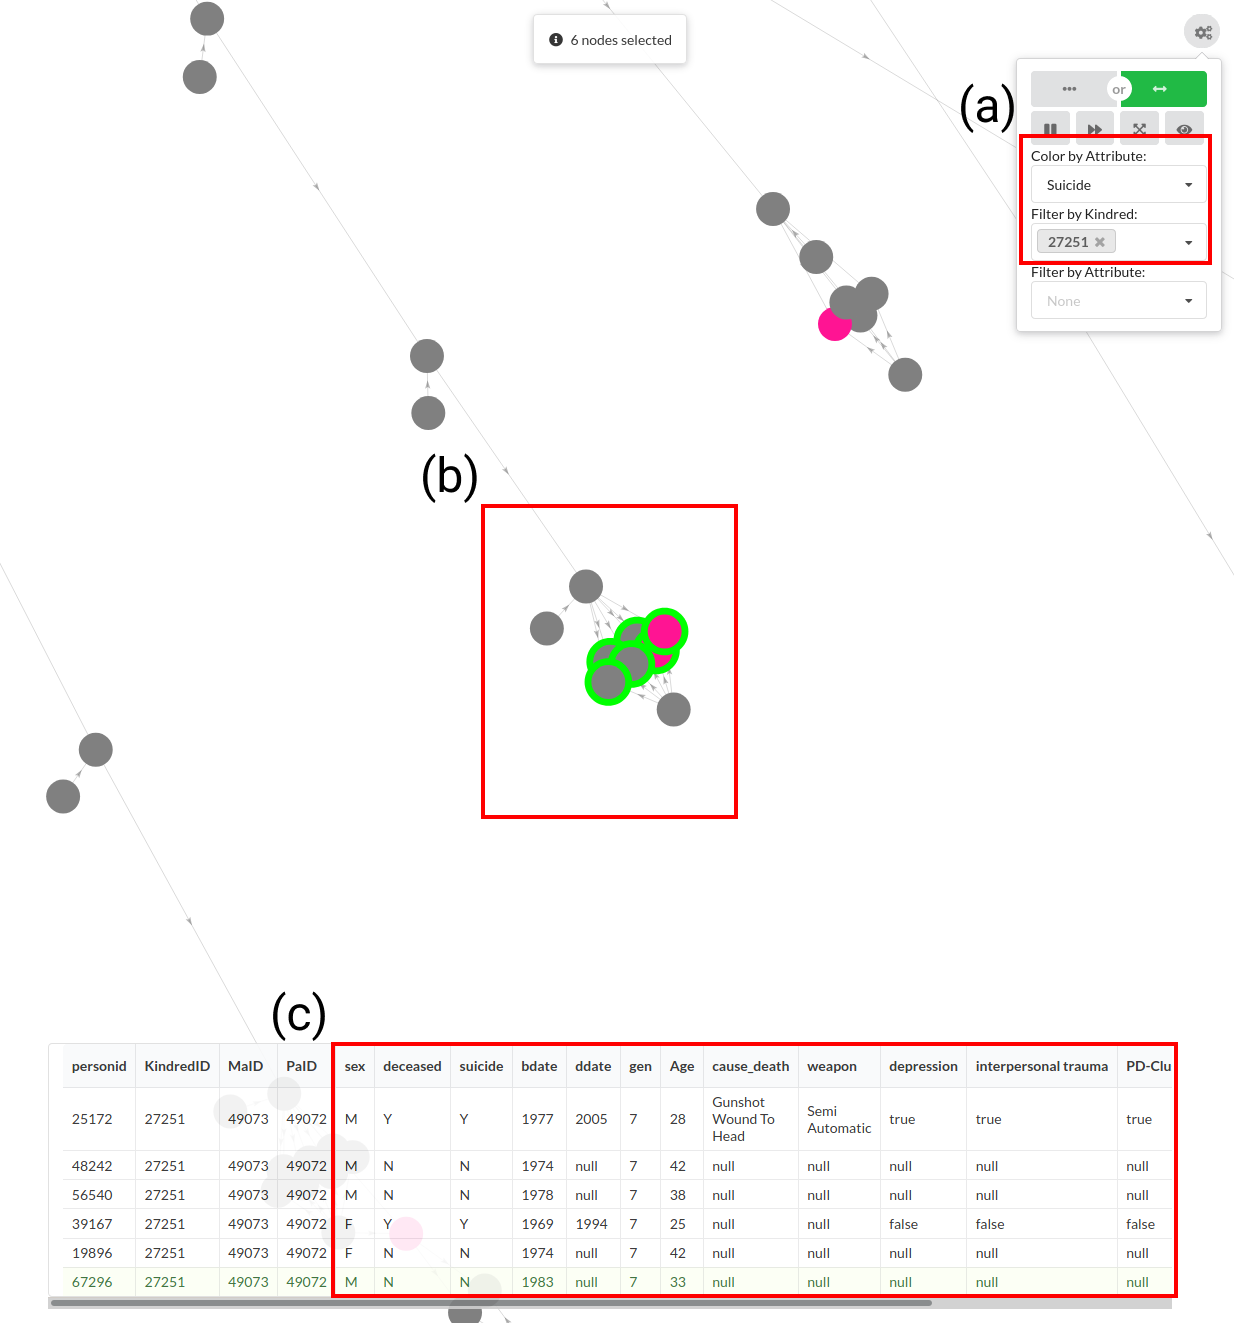
\includegraphics[width=\columnwidth]{pictures/comparison.png}
 \caption{A graph of a family within 2 suicide cases. (a) Colored by suicide cases and filtered by family 27251. (b) 2 suicide cases (colored in pink) with their siblings selected, which are highlighted in green. (c) Table of clinical attributes for the selected nodes.}
 \label{fig:comparison}
\end{figure}

\section{Conclusion}
A robust visualization system and domain experts are often needed to perform high-level visualization tasks on multivariate graph data. Nonetheless, a basic set of interactions and visualization techniques is often sufficient to perform several high-level visualization tasks as long as they can be broken down into low-level tasks defined by the Graph Task Taxonomy.


%\bibliographystyle{abbrv}
\bibliographystyle{abbrv-doi}
%\bibliographystyle{abbrv-doi-narrow}
%\bibliographystyle{abbrv-doi-hyperref}
%\bibliographystyle{abbrv-doi-hyperref-narrow}

\bibliography{template}
\end{document}
